\pagebreak
\begin{frame}{Gegenmaßnahmen}{Struktur}
    \begin{itemize}
        \item Stack-Schutz mit ``Canary'' (Zufallszahl)
        \item Safe Pointer Instrumentalisierung
        \item C Range Error Detector und Out Of Bounds Object
        \item Hardware-basierte Lösungen
        \item Statische Code-Analyse
        \item Betriebssystembasierte Ansätze
        \item Manuelles Buffer-Overflow Blocken (Input-Bereinigung)
    \end{itemize}
\end{frame}



\begin{frame}{Gegenmaßnahmen}{Code-Beispiel}
    \begin{center}
        %TODO: Besseres Beispiel finden.
        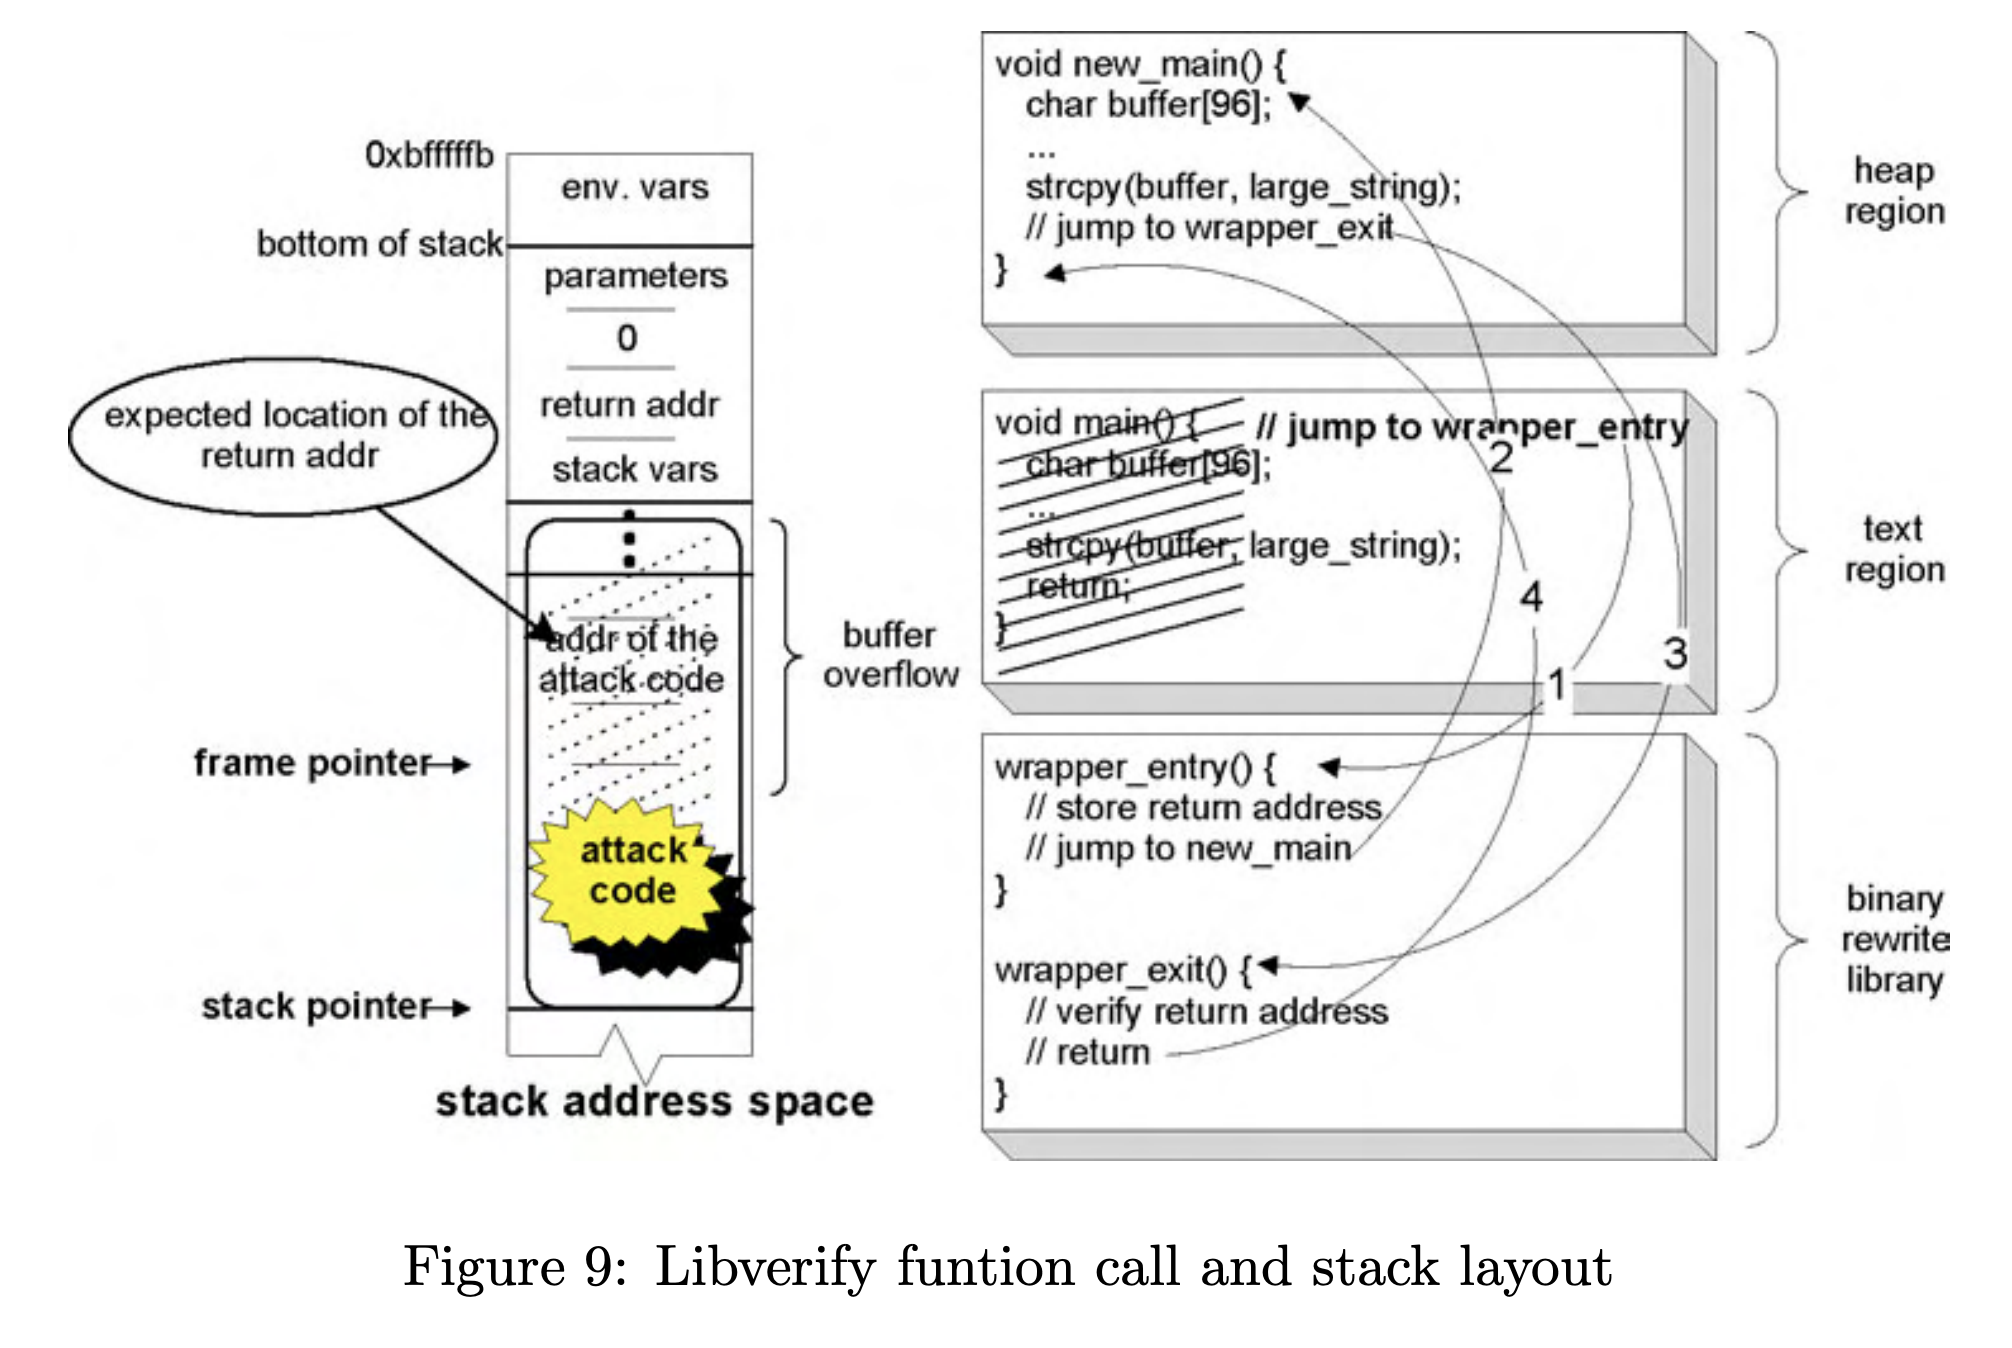
\includegraphics[width=\textwidth,height=0.75\textheight,keepaspectratio]{images/Libverify.png}
    \end{center}
\end{frame}

\begin{frame}{Gegenmaßnahmen}{Testen}
    \begin{itemize}
        \item Fuzzy Tests
        \item Spezifische Payloads
    \end{itemize}
\end{frame}